% Fig. 1: scope of Theorem 1 (single column, 246 pt = 8.646 cm wide), in the style of nested search-space
% diagrams: the same sets in three rows; a thick outline marks the set for which each statement holds.
%   N: noisy quantum systems that remove at most k bits of entropy per step (any size, any dynamics)
%   Q: quantum reservoirs, E: measurement-free error correction,
%   star: the explicit reservoir that reaches the lower bound (Fig. 4a).
% Row c chains the two bounds: e^{Omega(k)} <= max_Q W (row b) <= max_N W (Q lies in N) <= e^{O(k)} (row a).
% Palette of all figures (tikzstyle.tex): red = noise and the limit (upper bound, set N), blue = memory and the
% reservoir that attains it (lower bound, set Q), greys = neutral. The statements on the right carry the colour
% of the set they hold for.
\documentclass[border=0pt]{standalone}
% Shared TikZ style for the schematics. Same typeface, size (8 pt) and palette as figstyle.py:
% blue = memory / reservoir dynamics, red = noise and the limit, purple = input, greys = neutral.
\usepackage[T1]{fontenc}
\usepackage{helvet}
\renewcommand{\familydefault}{\sfdefault}
\usepackage{amsmath,amssymb,bm}
\usepackage{tikz}
\usetikzlibrary{arrows.meta,calc,decorations.pathreplacing,patterns.meta,shapes.geometric,shadows}
\definecolor{cInk}{HTML}{1A1A1A}
\definecolor{cBlue}{HTML}{3C7FE0}
\definecolor{cBlueDark}{HTML}{1D4C9C}
\definecolor{cBlueLight}{HTML}{8DB8F0}
\definecolor{cBlueFill}{HTML}{DDE9F9}
\definecolor{cRed}{HTML}{EF4B3B}
\definecolor{cRedDark}{HTML}{B8301F}
\definecolor{cRedFill}{HTML}{FCE3DE}
\definecolor{cPurple}{HTML}{9B4FE0}
\definecolor{cPurpleDark}{HTML}{6B2CAB}
\definecolor{cPurpleFill}{HTML}{EFE2FB}
\definecolor{cGreyDark}{HTML}{4A4A4A}
\definecolor{cGrey}{HTML}{8C8C8C}
\definecolor{cGreyLight}{HTML}{B4B4B4}
\definecolor{cGreyFill}{HTML}{EDEDED}
\definecolor{cShadow}{HTML}{B5B5B5}
\tikzset{
  every node/.style={font=\fontsize{8}{9.6}\selectfont},
  lbl/.style={font=\fontsize{8}{9.6}\selectfont},
  ttl/.style={font=\fontsize{8}{9.6}\selectfont,anchor=base west,inner sep=0pt},
  ttlr/.style={font=\fontsize{8}{9.6}\selectfont,anchor=base east,inner sep=0pt},
  wire/.style={line width=0.65pt,cInk},
  ublk/.style={draw=cInk,line width=0.6pt,fill=cBlue,rounded corners=1.6pt},
  iblk/.style={draw=cInk,line width=0.6pt,rounded corners=1.6pt,preaction={fill=cPurple},
    pattern={Lines[angle=55,distance=2.2pt,line width=0.85pt]},pattern color=white},
  nbox/.style={draw=cInk,line width=0.55pt,fill=cRed,rounded corners=1.1pt},
  feat/.style={draw=cInk,line width=0.6pt,fill=white,rounded corners=2pt,inner sep=1.6pt,
    minimum width=0.98cm,minimum height=0.44cm},
  legbox/.style={draw=cInk,line width=0.8pt,fill=white,rounded corners=2.4pt,
    drop shadow={shadow xshift=1.2pt,shadow yshift=-1.2pt,fill=cShadow,opacity=1}},
  arr/.style={line width=0.65pt,-{Stealth[length=3.6pt,width=3.2pt]}},
  brc/.style={decorate,decoration={brace,amplitude=2.6pt},line width=0.55pt},
}
\newcommand{\Discard}[3][cInk]{%
  \draw[line width=0.75pt,#1] (#2,{#3-0.1}) -- (#2,{#3+0.1});
  \draw[line width=0.75pt,#1] ({#2+0.05},{#3-0.064}) -- ({#2+0.05},{#3+0.064});
  \draw[line width=0.75pt,#1] ({#2+0.1},{#3-0.03}) -- ({#2+0.1},{#3+0.03});}
\providecommand{\ket}[1]{|#1\rangle}
\providecommand{\nrm}[2]{\lvert #1\rvert_{#2}}

\begin{document}
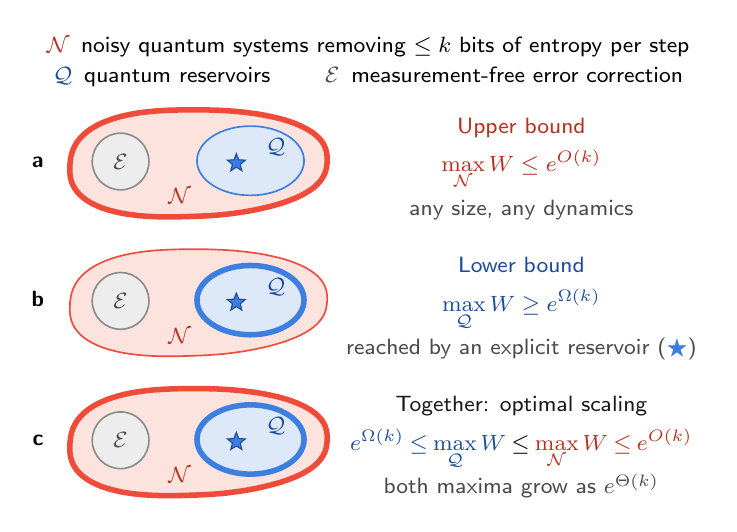
\begin{tikzpicture}[x=1cm,y=1cm]
\def\H{6.05}
\useasboundingbox (0,0) rectangle (8.646,\H);
% ------------------------------------------------------------------ the sets (relative to the centre of a row)
\def\XS{2.13}% centre of the sets
\def\XT{6.27}% centre of the statements
\def\Thick{2.0pt}\def\Thin{0.6pt}
\def\SetN{(1.672,0.000) -- (1.674,0.075) -- (1.667,0.133) -- (1.653,0.186) -- (1.631,0.235) -- (1.601,0.281) -- (1.564,0.324) -- (1.519,0.364) -- (1.469,0.401) -- (1.412,0.435) -- (1.350,0.467) -- (1.283,0.496) -- (1.212,0.523) -- (1.137,0.547) -- (1.058,0.569) -- (0.975,0.588) -- (0.889,0.606) -- (0.800,0.622) -- (0.707,0.635) -- (0.610,0.647) -- (0.508,0.657) -- (0.401,0.665) -- (0.287,0.671) -- (0.161,0.675) -- (0.000,0.676) -- (-0.162,0.676) -- (-0.288,0.673) -- (-0.404,0.668) -- (-0.512,0.661) -- (-0.614,0.651) -- (-0.710,0.639) -- (-0.802,0.624) -- (-0.889,0.606) -- (-0.971,0.586) -- (-1.048,0.563) -- (-1.119,0.538) -- (-1.185,0.511) -- (-1.246,0.482) -- (-1.302,0.450) -- (-1.352,0.417) -- (-1.398,0.381) -- (-1.438,0.344) -- (-1.474,0.305) -- (-1.505,0.264) -- (-1.531,0.220) -- (-1.553,0.174) -- (-1.570,0.125) -- (-1.583,0.070) -- (-1.592,0.000) -- (-1.595,-0.071) -- (-1.594,-0.127) -- (-1.588,-0.178) -- (-1.576,-0.227) -- (-1.559,-0.273) -- (-1.535,-0.318) -- (-1.505,-0.360) -- (-1.469,-0.401) -- (-1.426,-0.439) -- (-1.375,-0.476) -- (-1.318,-0.510) -- (-1.254,-0.541) -- (-1.184,-0.570) -- (-1.107,-0.595) -- (-1.023,-0.617) -- (-0.934,-0.637) -- (-0.839,-0.652) -- (-0.740,-0.665) -- (-0.635,-0.674) -- (-0.527,-0.680) -- (-0.413,-0.683) -- (-0.293,-0.684) -- (-0.163,-0.681) -- (-0.000,-0.676) -- (0.160,-0.669) -- (0.283,-0.660) -- (0.392,-0.650) -- (0.493,-0.637) -- (0.588,-0.624) -- (0.677,-0.609) -- (0.763,-0.593) -- (0.844,-0.575) -- (0.923,-0.557) -- (0.999,-0.537) -- (1.072,-0.516) -- (1.143,-0.493) -- (1.211,-0.468) -- (1.277,-0.442) -- (1.339,-0.413) -- (1.398,-0.381) -- (1.452,-0.348) -- (1.503,-0.311) -- (1.547,-0.271) -- (1.586,-0.228) -- (1.618,-0.182) -- (1.644,-0.131) -- (1.662,-0.074) -- cycle}
% #1, #2: line widths of N and Q
\newcommand{\Sets}[2]{%
  \filldraw[fill=cRedFill,draw=cRed,line width=#1,line join=round] \SetN;
  \filldraw[fill=cGreyFill,draw=cGrey,line width=\Thin] (-0.95,0.02) circle[radius=0.36];
  \filldraw[fill=cBlueFill,draw=cBlue,line width=#2] (0.70,0.03) ellipse[x radius=0.68,y radius=0.44];
  \node[star,star points=5,star point ratio=2.3,minimum size=6.8pt,inner sep=0pt,fill=cBlue,draw=cBlueDark,
    line width=0.4pt] at (0.52,0.0) {};
  \node[inner sep=0pt,text=cRedDark] at (-0.20,-0.42) {$\mathcal N$};
  \node[inner sep=0pt,text=cBlueDark] at (1.02,0.20) {$\mathcal Q$};
  \node[inner sep=0pt,text=cGreyDark] at (-0.95,0.02) {$\mathcal E$};}
\newcommand{\Statement}[4]{% title colour, title, formula, note; centred in the right column
  \node[anchor=base,inner sep=0pt,text=#1] at (\XT,0.38) {#2};
  \node[anchor=base,inner sep=0pt] at (\XT,-0.11) {#3};
  \node[anchor=base,inner sep=0pt,text=cGreyDark] at (\XT,-0.66) {#4};}
% ------------------------------------------------------------------ key
\node[anchor=base,inner sep=0pt] at (4.323,\H-0.32)
  {\textcolor{cRedDark}{$\mathcal N$}\, noisy quantum systems removing $\le k$ bits of entropy per step};
\node[anchor=base,inner sep=0pt] at (4.323,\H-0.70)
  {\textcolor{cBlueDark}{$\mathcal Q$}\, quantum reservoirs \qquad \textcolor{cGreyDark}{$\mathcal E$}\, measurement-free error correction};
% ------------------------------------------------------------------ a: upper bound for every member of N
\begin{scope}[shift={(\XS,4.33)}]
  \Sets{\Thick}{\Thin}
  \node[anchor=base,inner sep=0pt] at (-2.00,-0.05) {\textbf{a}};
\end{scope}
\begin{scope}[shift={(0,4.33)}]
  \Statement{cRedDark}{Upper bound}{\color{cRedDark}$\displaystyle\max_{\mathcal N}W\le e^{O(k)}$}{any size, any dynamics}
\end{scope}
% ------------------------------------------------------------------ b: lower bound for the class Q, reached by the star
\begin{scope}[shift={(\XS,2.56)}]
  \Sets{\Thin}{\Thick}
  \node[anchor=base,inner sep=0pt] at (-2.00,-0.05) {\textbf{b}};
\end{scope}
\begin{scope}[shift={(0,2.56)}]
  \Statement{cBlueDark}{Lower bound}{\color{cBlueDark}$\displaystyle\max_{\mathcal Q}W\ge e^{\Omega(k)}$}
    {reached by an explicit reservoir (\textcolor{cBlue}{$\bigstar$})}
\end{scope}
% ------------------------------------------------------------------ c: both bounds together (Q lies in N)
\begin{scope}[shift={(\XS,0.79)}]
  \Sets{\Thick}{\Thick}
  \node[anchor=base,inner sep=0pt] at (-2.00,-0.05) {\textbf{c}};
\end{scope}
\begin{scope}[shift={(0,0.79)}]
  \Statement{cInk}{Together: optimal scaling}
    {$\displaystyle\thickmuskip=4mu {\color{cBlueDark}e^{\Omega(k)}\le\max_{\mathcal Q}W}\le
      {\color{cRedDark}\max_{\mathcal N}W\le e^{O(k)}}$}
    {both maxima grow as $e^{\Theta(k)}$}
\end{scope}
\end{tikzpicture}
\end{document}
